\chapter{Referencial Teórico}
\label{cap:ref-teorico}
Neste capítulo é apresentado o referencial teórico utilizado neste trabalho. A Seção \ref{ref-teo:pac_rel_ver} discorre sobre \textit{pacote}, \textit{release} e \textit{versão}. A Seção \ref{ref-teo:prov_clie} distingue os termos \textit{provedor} e \textit{cliente}. A Seção \ref{ref-teo:semver} explica o que é \textit{Versionamento Semântico} e o \textit{SemVer} e como eles são utilizados no ecossistema do \gls{npm}. A Seção \ref{ref-teo:breaking_change} conceitua as \textit{breaking changes} e a Seção \ref{sec:related_works} apresenta os trabalhos relacionados.

\section{Pacote, \textit{Release} e Versão}
\label{ref-teo:pac_rel_ver}
Neste trabalho, o termo \textit{pacote} refere-se a um projeto de \textit{software} hospedado no \gls{npm}. Cada pacote contêm seu nome, seus arquivos e suas versões. O termo \textit{release} designa o estado de um pacote em um determinado instante. Uma \textit{release} é denotada por uma versão específica desse pacote, isto é, um conjunto de arquivos distintos das demais \textit{releases}. Por fim, o termo \textit{versão} é utilizado para especificar e distinguir um determinado estado de uma \textit{release}. Uma \textit{versão} é uma \textit{string} no padrão \textit{SemVer}, especificado na Seção \ref{ref-teo:semver}, que identifica unicamente uma determinada \textit{release} e é utilizada pelo \gls{npm} no arquivo \textit{package.json}. O arquivo \textit{package.json} é o arquivo de configuração das \textit{releases} que contém todas as informações pertinentes ao pacote naquela \textit{release}, tais como a lista de arquivos, o endereço do repositório, mas principalmente, sua versão única e todos os provedores com seus respectivos \textit{ranges} de versões que o cliente aceita. Ainda, o \textit{package.json} contém \textit{scripts} que podem ser executados e dois deles são os \textit{scripts install} e \textit{test}. Assim, o termo \textit{executar pacote/relese} se refere ao ato de executar os \textit{scripts install/test}.


%\begin{lstlisting}[style=bash, label=cod:install:provider]
%\end{lstlisting}
\section{Provedor e Cliente}
\label{ref-teo:prov_clie}
O provedor é pacote aquele que provê recursos ao cliente, ou seja, contém interfaces públicas para acesso às suas funcionalidades. O termo \textit{provedor} é também chamado de \textit{bibliotecas}. Por exemplo, suponha que o cliente execute o comando \texttt{npm install mocha}. Após a execução desse comando, o \gls{npm} salva o \textsf{mocha} no \textit{package.json} como um provedor. Assim, o pacote \textit{mocha} é um provedor direto, pois foi instalado diretamente pelo cliente. Entretanto, os provedores do \textit{mocha} também são instalados, mas de forma indireta pelo \gls{npm}. Estes outros pacotes são chamados de \textit{provedores indiretos} do cliente, pois não dependem que o cliente instale-os diretamente com o comando \textit{npm install}. A Figura \ref{fig:provider} mostra que o pacote \textit{mocha} é um provedor direto do \textit{client}, pois o \textit{client} requer o \textsf{mocha} para executar. Por sua vez, o pacote \textit{glob} é um provedor direto do \textit{mocha}, e um provedor indireto do pacote \textit{client}.

\begin{figure}
    \centering
    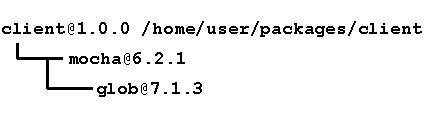
\includegraphics[scale=1.4]{figuras/provider_directly_undirectly.pdf}
    \caption{\textit{mocha} como provedor direto e \textit{glob} como indireto do \textit{client}}
    \label{fig:provider}
\end{figure}{}

O cliente é aquele que está acessando as interfaces públicas do provedor. Quando uma \textit{breaking change} é introduzida pelo provedor -- direto ou indireto --, essa \textit{breaking change} sempre se manifesta no cliente, causando o encerramento de sua execução. O cliente possui a responsabilidade de atualizar a versão de seus provedores no \textit{package.json} quando esses publicam uma \textit{release} com correções, enquanto o provedor possui a responsabilidade de indicar o nível de compatibilidade que sua nova \textit{release} está introduzindo \cite{teorical_reference:semver}, ou seja, se sua \textit{release} é ou não compatível.

\section{Versionamento Semântico e \textit{SemVer}}
\label{ref-teo:semver}

O Versionamento Semântico\footnote{https://semver.org} é um padrão para versionamento de \textit{releases} de um projeto que considera o tipo de alteração introduzida na \textit{release}. As regras do Versionamento Semântico foram idealizadas por Tom Preston-Werner -- criador do \textit{GitHub} -- que incentiva todos os desenvolvedores à utilizarem esse padrão, uma vez que suas regras são baseadas em práticas comuns já utilizadas em projetos \cite{teorical_reference:semver}. Uma \textit{string} de versão no padrão do Versionamento Semântico possui os níveis \textit{<MAJOR>.<MINOR>.<PATCH>}\footnote{a \textit{string} pode ser estendida para versões \textit{beta, alpha, pre}, entre outros, tal como \textit{x.y.z-beta.0}}, que devem ser incrementados, quando o desenvolvedor publicar uma \textit{release}, de acordo com o seguinte critério:

\begin{itemize}
    \item \textit{MAJOR}: deve ser incrementado quando a \textit{release} introduz \textit{breaking changes};
    \item \textit{MINOR}: incrementado quando for adicionado melhorias/novas funcionalidades que mantenham a compatibilidade com as \textit{releases} anteriores; e
    \item \textit{PATCH}: deve ser incrementado quando a \textit{release} contém correção de \textit{bugs}.
\end{itemize}{}

Dessa maneira, se um projeto contém a sua última \textit{release} versionada como \textit{2.1.0}, por exemplo, o seu nível \textit{major} é o 2; o \textit{minor}, 1; e o \textit{patch}, 0. Ao publicar uma nova \textit{release}, se essa contiver uma \textit{breaking change}, então deverá ser publicada com a versão \textit{3.0.0}; se for introduzida uma nova funcionalidade, \textit{2.2.0}; se houver uma correção de \textit{bugs}, \textit{2.1.1}; e se introduzir os três tipos de alterações, o nível \textit{major} deverá ser incrementado, uma vez que uma \textit{breaking change} é a alteração que mais afeta o cliente.

O \textit{SemVer} é uma \textit{string} de versionamento que especifica um intervalo de versões, ou um \textit{range}. Com o \textit{SemVer} é possível especificar quais são as \textit{releases} que o cliente aceita do seu provedor. Há vários padrões de \textit{range}\footnote{https://github.com/npm/node-semver\#ranges} especificados pelo \textit{SemVer}, mas os mais comuns, utilizados pelo \gls{npm}, são:

\begin{itemize}
    \item \textit{X-Ranges (*)}: este \textit{range} especifica para o \gls{npm} que o cliente aceita qualquer nova \textit{release} do provedor, até mesmo as \textit{releases} com \textit{breaking changes};
    \item \textit{Caret Ranges (\textasciicircum)}: este é o \textit{range} mais comum e o padrão do \gls{npm}. Com o \textit{Caret Range}, o cliente especifica que o \gls{npm} só deve descarregar novas \textit{releases} do provedor que contenham novas funcionalidades e correções de erros, mas que não contenham \textit{breaking changes}, ou seja, o cliente aceita todas as \textit{releases} das quais foram atualizadas os níveis \textit{patch} ou \textit{minor};
    \item \textit{Tilde Ranges (\textasciitilde)}: neste \textit{range}, o cliente especifica para o \textit{NPM} que somente as \textit{releases patch} do provedor são aceitas.
\end{itemize}{}

O \gls{npm} utiliza o padrão \textit{SemVer} no arquivo \textit{package.json} pois, através do \textit{SemVer}, o cliente pode decidir o quão flexível será receber as futuras \textit{releases} dos provedores \cite{decan}. Por exemplo, ao executar o \textit{npm install express --save}, para instalar o provedor \textit{express}\footnote{https://www.npmjs.com/package/express} por exemplo, o \gls{npm} -- além de descarregar esse provedor -- irá salvar no \textit{package.json} o nome do provedor com sua versão atual em modo \textit{range}, de acordo com a Figura \ref{fig:dep_express}.

\begin{figure}
    \centering
    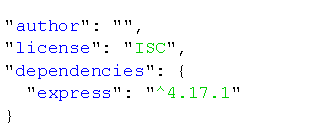
\includegraphics[scale=1.3]{figuras/dependencies_express.pdf}
    \caption{Modo como o \gls{npm} salva no \textit{package.json} a versão de uma dependência}
    \label{fig:dep_express}
\end{figure}{}

Com a informação do \textit{range} do provedor no \textit{package.json}, o \gls{npm} sempre irá resolver o \textit{range} e descarregar as \textit{releases} mais recentes que são aceitas pelo \textit{range SemVer} especificado pelo cliente. \textit{Resolver o range} significa recuperar todas as versões do provedor e selecionar a mais recente que é aceita pela \textit{string SemVer} especificada pelo cliente. Por padrão, o \gls{npm} especifica o \textit{Caret Range}, mas o cliente pode especificar outro \textit{range} manualmente no \textit{package.json} ou pode utilizar a opção \textit{--save-exact} para especificar a versão sem o \textit{range}, fazendo com que o \gls{npm} sempre instale essa versão específica.

\section{\textit{Breaking Change}}
\label{ref-teo:breaking_change}
Uma \textit{breaking change} é uma alteração no provedor que produz defeitos nos clientes \cite{teorical_reference:semver}. As \textit{breaking changes} surgem quando o provedor, que previamente era utilizado com sucesso pelo cliente, publica uma \textit{release} que causa no cliente um comportamento inesperado, resultando em um erro. Durante o desenvolvimento de \textit{software}, os provedores precisam introduzir \textit{breaking changes}, pois quando só há \textit{releases} compatíveis com versões anteriores, o \textit{software} perde muitas oportunidades de evolução \cite{teorical_reference:bc_2}. Desta maneira, as \textit{breaking changes} são importantes para a evolução de um \textit{software}, uma vez que apenas \textit{releases} compatíveis podem estagnar o \textit{software}, limitando sua evolução. Assim, as \textit{breaking changes} também são sinônimos de evolução. Exemplo disso é o \textit{Node.js}, que publica uma \textit{release} incrementando o nível \textit{major} a cada 6 meses\footnote{https://github.com/nodejs/node\#release-types}. Desta maneira, introduzir \textit{breaking changes} em níveis \textit{major} permite que os \textit{softwares} evoluam sem manter-se presos à versões anteriores.

Para evitar que os impactos de uma \textit{breaking change} afetem os clientes, os provedores publicam suas \textit{releases} com \textit{breaking changes} incrementando o nível \textit{major} da sua nova versão, seguindo a regra do Versionamento Semântico. Dessa maneira, os clientes de versões prévias que especificaram o provedor com o \textit{range caret} -- \textit{range} especificado por padrão pelo \gls{npm} -- ou o \textit{range tilde}, não serão afetados por uma \textit{breaking change}. Porém, uma \textit{breaking change} pode ser introduzida erroneamente quando é atualizado os níveis \textit{minor} ou \textit{patch}. Dessa maneira, o problema das \textit{breaking changes} está no fato do provedor introduzi-las em \textit{releases minor} ou \textit{patch}, resultando em defeitos nos clientes.

\subsection{Casos particulares de \textit{breaking changes}}
Além de alterações que resultam em \textit{breaking changes}, há algumas alterações que são causadas por provedores mas que, nessa pesquisa, não serão consideradas como \textit{breaking changes}, uma vez que esses casos não significam que o provedor contenha um erro ou não fazem parte do ecossistema do \textit{npm} . Essas alterações são:

\begin{itemize}
    \item Alterações da versão do \textit{Node.js}: o \textit{Node.js} atualizou o seu nível \textit{major} de \textit{0.x} para \textit{7.x} em apenas 3 anos\footnote{https://nodejs.org/en/download/releases}, mas isso não significa que os pacotes evoluíram seus códigos sempre para a última \textit{release} do \textit{Node.js}, e o inverso é valido, ou seja, os pacotes podem ter evoluído seus códigos na mesma frequência do \textit{Node.js}. Por exemplo, considere um cliente executando no \textit{Node.js 0.x} com um provedor que evoluiu seu código para a sintaxe do \textit{Node.js 6.x}, que não é aceita no \textit{Node.js 0.x}. Desta maneira, não há uma versão do \textit{Node.js}  na qual seja possível executar o cliente sem que no provedor seja manifestado um erro. Assim, erros nos provedores ocasionados por versões do \textit{Node.js} não serão considerados como \textit{breaking changes}, pois o erro foi causado pelo \textit{Node.js}, que não reconhece a sintaxe, e não pelo provedor;

    %\item Exclusão de uma \textit{release}/\textit{provedor} do \gls{npm}: pelas regras do \gls{npm}, uma \textit{release} só pode ser removida até 72 horas após ter sido publicada\footnote{https://docs.npmjs.com/cli/unpublish\#description}. Entretanto, quando uma \textit{release} é removida do \gls{npm} e o cliente especificou aquela \textit{release}, isso gera um erro no \textit{script install}. Assim, o erro é causado pelo \gls{npm} que não consegue encontrar a \textit{release}, e não pelo provedor. No caso do provedor ter sido removido do \gls{npm} o caso é o mesmo: um provedor só pode ser removido após 72 horas. Entretanto, anterior ao acontecimento do \textit{left-pad}, os pacotes -- e \textit{releases} também -- podiam ser removidos do \gls{npm} em qualquer circunstância. Por isso, quando um pacote removido do \gls{npm} causar um erro, não será considerado como uma \textit{breaking change}.
    \item Alterações em serviços externos: os provedores podem fazer uso de sistemas externos, tais como acesso à \textit{API's} de sites e sistemas, e recuperar dados dessas. Entretanto, ao longo do tempo, naturalmente, essas \textit{API's} podem alterar seus dados, o que gera inconsistências em seus clientes. Mas esse tipo de erro não é considerado como uma \textit{breaking change}, uma vez que esse caso não faz parte do ecossistema do \gls{npm}; e
    \item Cliente aceita \textit{releases major} do provedor: quando o cliente especifica em seu \textit{package.json} que aceita qualquer \textit{release} do provedor, através de um \textit{X-range}, o cliente então também está aceitando \textit{releases} que introduziram \textit{breaking changes}. Por isso, quando um cliente for impactado por uma \textit{breaking change} no provedor, e que foi corretamente introduzida em uma \textit{release major}, significa que o problema está no cliente que aceitou a \textit{breaking change} mas não a tratou.
\end{itemize}{}

\section{Trabalhos Relacionados}
\label{sec:related_works}

O trabalho de \citeonline{teorical_reference:bc_1} propõe detectar \textit{breaking changes} em pacotes \textit{Javascript} por meio de uma ferramenta que foi desenvolvida para esse propósito. Para esse trabalho, foram escolhidos três provedores com um total de 3000 pacotes clientes. Os provedores foram escolhidos pelo critério de popularidade no \gls{npm}, isto é, os pacotes que possuíam mais clientes, resultando nos pacotes \textit{lodash}, \textit{underscore} e \textit{bluebird}. Já a escolha dos pacotes clientes se deu recuperando 1000 pacotes, aleatoriamente, da página de cada provedor.\footnote{https://www.npmjs.com/browse/depended/lodash}

Para identificar as \textit{breaking changes}, o código dos provedores, versão por versão, foi transformado em um \textit{AST} e extraído apenas as \textit{APIs}. Então, foi possível verificar entre duas versões do provedor se houve alguma alteração no nome/lista de parâmetros das \textit{APIs}. Nos clientes o processo não foi diferente: o código dos clientes foi transformado em uma \textit{AST} e verificado quais funções os clientes usam dos provedores e se essas são as que contêm \textit{breaking changes} que foram detectadas no código dos provedores. Também, foi verificado manualmente nas documentações dos provedores pelos casos de \textit{breaking changes} que estavam documentadas para verificar se a ferramenta encontrava corretamente esses casos. Então, dos três pacotes, resultando em 231 \textit{releases}, foi constatado um total de 21 (9.1\%) de versões com identificadas com \textit{breaking changes} pela ferramenta e foi constatado que a ferramenta é capaz de detectar corretamente entre 43\% e 80\% dos casos de \textit{breaking changes} para um determinado projeto.

Entretanto, a ferramenta desenvolvida por \citeonline{teorical_reference:bc_1} verifica apenas alterações de \textit{API's} dos provedores, limitando-se às alterações dos nomes e da lista de parâmetros, uma vez que alterações no tipo dos parâmetros não foram consideradas, nem qualquer outra categoria de \textit{breaking change}. Também, a ferramenta foi aplicada apenas aos três pacotes com mais clientes do \textit{npm}. A proposta do presente trabalho consiste em detectar qualquer categoria de \textit{breaking changes} introduzida pelos provedores e também propõe executar os \textit{scripts} de teste dos clientes, para que seja possível encontrar \textit{breaking changes} em qualquer provedor, direto ou indireto.

O trabalho de \citeonline{noregrets2018} apresenta uma ferramenta para detectar \textit{breaking changes} entre duas \textit{releases} de um provedor. É usada uma técnica de \textit{teste de regressão de tipo}, que consiste em verificar o tipo do objeto retornado por uma \textit{API} pública dos provedores, além de detectar alterações na assinatura da \textit{API}. A vantagem desse tipo de teste é que, além de alterações de \textit{API}, é possível detectar \textit{breaking changes} mesmo que o teste do cliente execute com sucesso. Assim, foi implementado um mapeamento de execuções para o provedor e o tipo de objeto que foi retornado daquela execução. A ferramenta desenvolvida se chama \textit{NoRegrets}.\footnote{https://github.com/cs-au-dk/NoRegrets}

Para testar a ferramenta \textit{NoRegrets}, foram selecionados 12 pacotes dentre os mais populares do \gls{npm}, ou seja, dentre os que mais possuíam clientes. Também foram recuperados alguns testes dos seus clientes. Para cada provedor, foi recuperada sua \textit{release major} mais recente e todas as suas \textit{releases patch/minor} dentre o \textit{range} da respectiva \textit{release major}. Já os clientes com testes foram escolhidos apenas os quais usavam o \textit{mocha}, assim, simplificando a análise. Então os testes dos clientes foram executados para cada uma das \textit{releases} dos provedores. A ferramenta \textit{NoRegrets} reportou 9.4\% de \textit{releases} com alterações nos tipos retornados pela \textit{API's} públicas dos provedores. Por fim, em 90\% dos casos a ferramenta \textit{NoRegrets} classifica corretamente se uma determinada \textit{release} do provedor deve ser publicada com a versão \textit{major, minor} ou \textit{patch}.

A ferramenta \textit{NoRegrest} apenas verifica \textit{breaking changes} relacionadas à alterações de objetos retornados pelas \textit{API's} dos provedores. Qualquer outra categoria de \textit{breaking change} não é verificada. O presente trabalho propõe detectar qualquer categoria de \textit{breaking change} e categorizá-las.